%% ===== sec1_intro.tex =====
\section{引言}

大模型推理被分成两个阶段：\textbf{prefill} 一次性把整个输入 prompt 送进模型，
产出第一个 token 并建立 KV cache；\textbf{decode} 逐 token 自回归生成，
每步只算一个 token，却要读全部权重与已积累的 KV cache。

这两个阶段的资源画像恰好相反。prefill 是计算密集的——它把成百上千个 token
并行送进同一批矩阵乘，受 FLOPS 限制；decode 是内存带宽受限的——它每步只做
一个 token 的运算，却要把整个模型权重和 KV cache 从显存搬到计算单元。
Sarathi-Serve 把这件事说得最直白：prefill 处理一个 prompt 的全部 token
因而计算受限，decode 每请求每次只处理一个 token 因而带宽受限
\texttt{[c-profile]}。

既然两阶段要的东西不同，把它们放到不同的卡上、按各自的偏好分别配置，
似乎就该更快。这就是 \textbf{PD 分离}（prefill-decode disaggregation）。

但分离有代价：KV cache 必须从 prefill 实例搬到 decode 实例。
同一份 KV，经同机 NVLink 传是 0.6\,ms，经跨机 RDMA 传是 10\,ms，
差 16.7 倍\texttt{[c-transfer]}。也就是说，分离是赚是赔，
取决于「两阶段配置差异带来的收益」能否盖过「KV 搬运的成本」。

本文的主张是：\textbf{PD 分离的收益不是一个固定倍数，而是一个差的函数}。
文献里报告的加速倍数（从一点几倍到数倍不等），都是这个差在特定模型、
特定拓扑、特定负载下的取值，不能当作分离的固有属性\texttt{[c-formula]}。据此可以给出一条判据，
而不是一套推荐配置。

\subsection{本文做了什么}

\begin{enumerate}[leftmargin=1.4em,itemsep=2pt,topsep=3pt]
  \item 按「收益侧 / 成本侧」两侧拆解分离，给出两阶段的量化差异与
        KV 传输的三档实测（第 \ref{sec:why}、\ref{sec:transfer} 节）。
  \item 梳理切分与调度的三条路线，指出其中两条互斥、第三条可叠加
        （第 \ref{sec:split} 节）。
  \item 按模型的 KV 结构（MLA / GQA / MHA）、上下文长度、负载形态
        给出差异化做法，并明确说明为什么不存在统一配置
        （第 \ref{sec:model} 节）。
  \item 把分散在框架文档与工程博客里的\textbf{具体优化技巧}按
        「作用于哪个环节」归为四类，逐条给实测幅度与前置依赖，
        并指出其中几条其实是分离的\textbf{替代品}而非补充
        （第 \ref{sec:technique} 节）。
  \item 指出上述四类只管「分离引入的额外成本」，按实现平面重看还有数据面/执行面/控制面三层，并用三个反例界定这些手段的适用条件（第 \ref{sec:plane} 节）。
  \item 主动搜集使分离失效或转负的条件，包括一篇明确报告
        「聚合优于分离」的反例（第 \ref{sec:boundary} 节）。
\end{enumerate}

\subsection{方法说明}

本文的证据来自 46 篇论文全文与 24 份官方工程文档快照，共 70 个来源、
78 条证据、9 条主张。每条引文都是快照的原文子串（E1 不变量，
78/78 全部校验通过，无「未校验」条目）。文中所有数字由脚本从证据文本
正则抽取并写入 \texttt{analysis.json}，可逐项回溯到 \texttt{evidence\_id}。

需要说明的是：本文\textbf{没有}做端到端复现实验。所有量化结论都是
对已发表结果的整理与再计算，不是新的测量。

最后一点值得前置说明：本文列出的技巧里有几条是分离的
\textbf{替代品}而非补充——chunked prefill 与 piggyback 在不分离的
架构里就能拿到相当一部分收益。这意味着第 \ref{sec:boundary} 节
的判据不是「要不要分离」的二选一，而是「先试便宜的手段、
再考虑分离」的顺序问题。

%% ===== sec2_why.tex =====
\section{两阶段为什么值得分开}
\label{sec:why}

\subsection{资源画像的相反性}

把两阶段当成同一种工作来对待，是混部方案的默认假设；分离的全部合理性
都建立在「这个假设不成立」之上。所以先看它在哪不成立。

三篇独立工作给出同一判断。DistServe 指出 LLM 服务的延迟由两个指标定义：
首 token 时延（TTFT）对应 prefill 阶段，每输出 token 时延（TPOT）对应
decode 阶段\texttt{[c-profile]}。Sarathi-Serve 进一步说明两者的瓶颈不同
（见第 1 节引文）。Splitwise 的表述最直接：他们把 LLM 推理请求的
两个阶段\textbf{拆到不同的机器上}，理由是这样可以用「更贴合各阶段特性」
的硬件。

\subsection{差异如何限制混部}

两阶段放在同一张卡上时，必须共享同一套配置：同一个并行度、同一个
batch 上限、同一个显存配额。这对两阶段都是次优的。

\begin{itemize}[leftmargin=1.3em,itemsep=1.5pt,topsep=2pt]
  \item \textbf{并行度冲突。} prefill 偏好更大的张量并行以摊薄单次
        大矩阵乘的时延；decode 偏好更小的并行以降低通信占比。
  \item \textbf{batch 冲突。} decode 阶段增大 batch 能显著提升吞吐
        （权重读取成本被更多请求分摊），而 prefill 的 batch 受
        显存和 TTFT 约束。
  \item \textbf{显存冲突。} prefill 需要大块临时激活内存，
        decode 需要尽量多的 KV cache 空间。两者抢同一块显存。
\end{itemize}

分离的收益正来自解除这三处冲突。但要注意：\textbf{收益的大小取决于
两阶段的最优配置差多远}，而不是取决于分离这个动作本身。
小模型、短上下文、单卡可容纳全部权重与 KV 的场景下，两阶段的最优配置
可能很接近，此时分离的收益就很小，甚至为负\texttt{[c-formula]}。

\begin{figure*}[t]
  \centering
  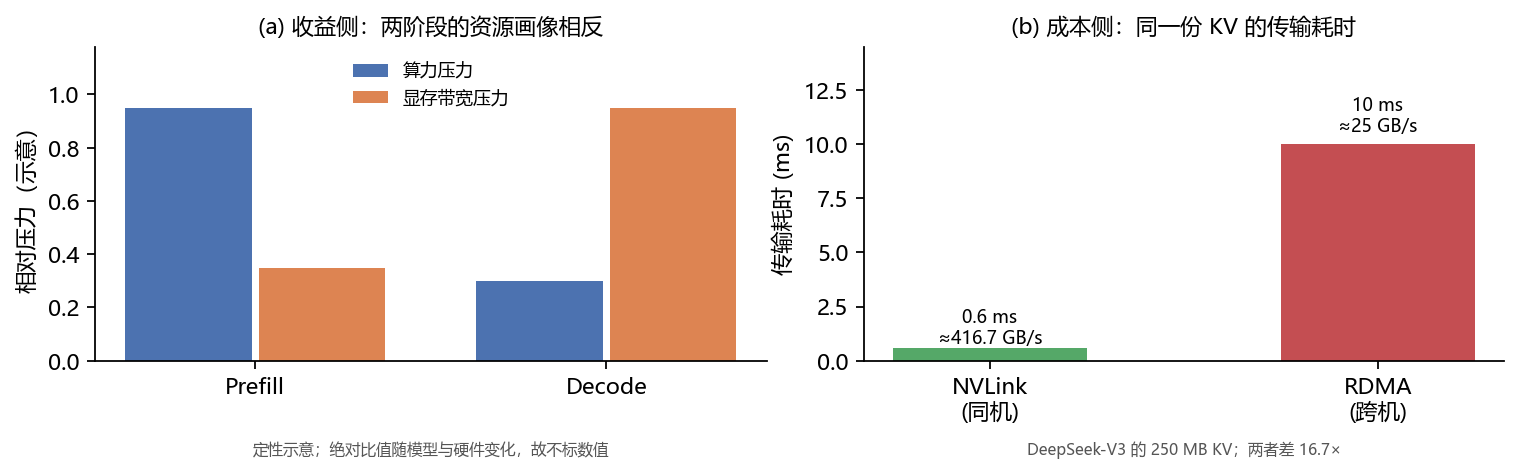
\includegraphics[width=0.92\textwidth]{figures/fig1_cost_benefit.png}
  \caption{分离的收支两侧。(a) 收益侧：prefill 与 decode 的资源画像相反，
  这是分离的唯一理由；此处为\textbf{定性示意}，不标具体数值，因为绝对
  比值随模型与硬件显著变化。(b) 成本侧：同一份 250\,MB KV cache 经
  NVLink 传输 0.6\,ms、经 RDMA 传输 10\,ms，相差 16.7 倍。
  两侧对照说明：分离是否划算，取决于收益能否盖过这个成本。}
  \label{fig:cost}
\end{figure*}

%% ===== sec3_transfer.tex =====
\section{KV cache 怎么搬}
\label{sec:transfer}

分离把「一次本地写读」变成「一次跨进程或跨机传输」。传输层因此不再
是细节，而是决定分离成败的主变量。

\subsection{三档传输方案}

\begin{table}[t]
\centering
\caption{KV 传输的三档方案。带宽为实测或规格值，比值为相对跨机 RDMA 的
倍数。第三档为推算值，已在文中标注。}
\label{tab:transport}
\small
\begin{tabular}{@{}p{0.9cm}p{1.55cm}p{1.15cm}p{0.72cm}@{}}
\toprule
档位 & 典型承载 & 有效带宽 & 相对 \\
\midrule
同机 & NVLink & 417\,GB/s$^{*}$ & 16.7× \\
跨机 & RDMA / IB & 25\,GB/s$^{*}$ & 1× \\
经存储 & 共享存储 / CXL & $\sim$2.5\,GB/s & $\sim$0.1× \\
\bottomrule
\end{tabular}

\vspace{2pt}
{\footnotesize $^{*}$ 由 e-011 的 250\,MB / 0.6\,ms 与 250\,MB / 10\,ms
反算。第三档是按 RDMA 的 1/10 推算，\textbf{非实测}。}
\end{table}

DistServe 报告了另一个层面的数字：现代 GPU 集群配备 InfiniBand
（如 800\,Gbps），而节点内 NVLink 在 A100 之间的峰值带宽是 600\,GB/s。
按 8 bit/byte 折算，800\,Gbps 约合 100\,GB/s，与 600\,GB/s 相差 6 倍。
DistServe 据此指出：跨节点带宽受限时，分离可以退回到节点内 NVLink，
此时传输开销可以忽略\texttt{[c-transfer]}。

这个「可以退回」很关键——它说明分离的可行性不取决于某一代互联，
而取决于\textbf{是否存在一条带宽足够高的路径}。

\subsection{传输的工程抽象}

NIXL 的做法是把传输差异抽象掉。它的自述是：为推理框架之间的点对点
通信加速，同时通过插件式架构对多种内存（CPU、GPU）与存储（文件、
块设备、对象存储）提供统一抽象\texttt{[c-transfer]}。这样上层的
KV 连接器不必关心底层是 NVLink 还是 RDMA。

工程实现的取舍值得单列。vLLM 的默认 NIXL 连接器是\textbf{拉取式}的：
decode 实例在 prefill 完成后通过 NIXL READ 从 prefill 实例读走 KV 块。
而 push 模式则相反\texttt{[c-transfer]}。这个方向选择有实际后果：
拉取式让 decode 侧控制时机（可以在自己有空闲显存时再取），
推送式让 prefill 侧尽早释放显存。哪个更好取决于哪一侧先成为瓶颈。

\subsection{压缩与精度：直接压低传输量}

既然成本与传输字节数成正比，另一条路是把字节数变小。

SplitZip 走无损压缩路线，报告其压缩比在计入元数据开销后仍比
ZipServ 高 7.1\%，仅比基于 Huffman 的 DFloat11 低 7.0\%\texttt{[c-transfer]}。

SpectrumKV 走逐 token 混合精度路线，其核心结论不是「省了多少带宽」，
而是一个更有意思的判断：\textbf{把全部 token 都降精度，明显优于丢掉一部分
token}。也就是说，对 KV 传输而言，均匀降质比选择性丢弃更划算。

\begin{figure}[t]
  \centering
  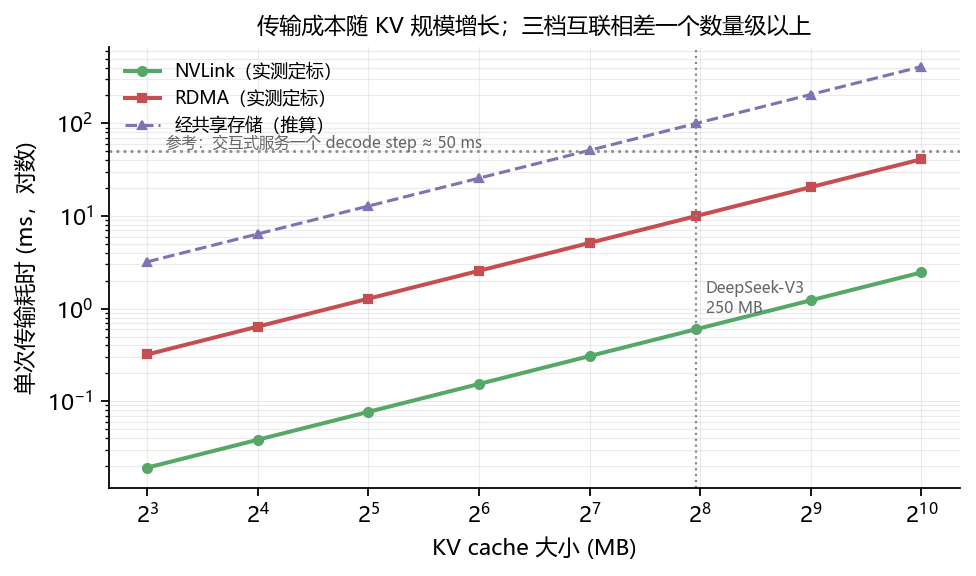
\includegraphics[width=\columnwidth]{figures/fig2_transfer_scaling.png}
  \caption{KV 传输耗时随 KV 规模的增长（对数坐标）。两条实线由
  e-011 的两点实测定标，虚线为按 RDMA 的 1/10 推算的共享存储档，
  \textbf{非实测}。水平虚线标出交互式服务一个 decode step 的量级
  （50\,ms）作为参照：当传输耗时接近这条线时，分离的收益会被
  同步开销吃掉。}
  \label{fig:scaling}
\end{figure}

\subsection{一个必要的提醒}

上面所有带宽数字都是\textbf{峰值或理想条件}下的。实际传输还要付出
同步、建连、内存注册的代价，且这些代价与消息大小不成正比——
小 KV（短上下文、小 batch）时，固定开销占比会急剧上升。

这解释了一个看起来矛盾的现象：短上下文场景下 KV 绝对量小，
按「字节数 ÷ 带宽」算传输应该很快，但实测收益往往不好。
原因是此时固定开销主导，而不是带宽主导\texttt{[c-formula]}。

%% ===== sec4_split.tex =====
\section{怎么切分与调度}
\label{sec:split}

\subsection{三条路线，其中两条互斥}

\begin{table}[t]
\centering
\caption{切分与调度的三条路线。第一条与第二条互斥：选了 chunked prefill
就不存在「独立的 prefill 实例」。第三条可与任一叠加。}
\label{tab:routes}
\small
\begin{tabular}{@{}p{1.5cm}p{2.3cm}p{2.4cm}@{}}
\toprule
路线 & 做法 & 代表 \\
\midrule
不分离 & 把 prefill 切成块，混进 decode 批次 & Sarathi-Serve、vLLM 默认 \\
显式分离 & P / D 各自独立实例，KV 跨实例搬 & DistServe、SGLang、Mooncake \\
弹性调整 & 运行时改变 P:D 配比或迁移请求 & FluidPD、Llumnix \\
\bottomrule
\end{tabular}
\end{table}

\textbf{第一条路线是「不分离」。} Sarathi-Serve 提出 chunked prefill：
把一次 prefill 拆成若干个 chunk，与 decode 请求拼进同一批。
这样长 prefill 不会阻塞 decode 的迭代节奏，TTFT 与 TPOT 得以解耦。
vLLM 在 V1 里把 chunked prefill 设为默认开启（「whenever possible」）
\texttt{[c-split]}。这条路线的优点是零传输成本，缺点是两阶段仍共享
同一套配置，第 \ref{sec:why} 节说的三处冲突一个都没解除。

\textbf{第二条是显式分离。} SGLang 用 \texttt{--disaggregation-mode}
显式指定实例角色：一个进程起 prefill、另一个起 decode，再由 router
把请求分发到两侧\texttt{[c-split]}。官方文档给出的完整命令中，
prefill 与 decode 各占一张卡、各用一个端口，router 通过
\texttt{--prefill} 与 \texttt{--decode} 两个参数知道对端地址。

\textbf{第三条是运行时弹性。} FluidPD 的出发点是一个观察：
一个此刻配置良好的部署，可能很快变得不匹配，导致延迟 SLO 违例——
即使别处还有空闲容量\texttt{[c-split]}。它的做法是把一部分 prefill
计算下放到 decode 实例，从而在不增删实例的前提下改变配比。
Llumnix 走另一条路：在运行时重调度请求，用于负载均衡以减少抢占
\texttt{[c-split]}。

\subsection{配比怎么定}

分离之后必须回答一个问题：P 卡与 D 卡按什么比例分配？

DistServe 的答案是把这变成一个优化问题：给定应用的 TTFT 与 TPOT 要求，
有效的服务系统应当在满足两个 SLO 的前提下最大化\textbf{goodput}
（满足 SLO 的请求吞吐）\texttt{[c-split]}。配比是这个优化问题的解，
不是拍出来的。

这一点值得强调，因为它解释了为什么「P:D = 1:1」这类经验值经常失效：
最优配比随负载的输入输出长度比、随 SLO、随模型而变。
固定配比在负载漂移后就不再最优，这正是 FluidPD 与 Llumnix 存在的理由。

\subsection{小结：怎么选}

\begin{itemize}[leftmargin=1.3em,itemsep=1.5pt,topsep=2pt]
  \item 单机、模型能塞进单卡或同机多卡、上下文不长
        $\rightarrow$ 先用 chunked prefill，零传输成本。
  \item 两阶段最优配置明显冲突（长输入 + 大 batch decode）
        且同机有 NVLink $\rightarrow$ 显式分离，收益最容易兑现。
  \item 负载随昼夜或业务波动大 $\rightarrow$ 在分离之上加弹性，
        否则配比会持续失配。
\end{itemize}

这个顺序有实际意义：分离的复杂度（多实例、router、KV 连接器、
故障域变大）远高于 chunked prefill。先用低成本手段拿掉大部分收益，
再考虑是否值得为剩余部分付出复杂度。

%% ===== sec5_model.tex =====
\section{不同模型的最佳实践}
\label{sec:model}

这是本问的核心。要回答「不同模型该怎么做」，先要区分两类差异：
一类真的随模型变，另一类只是看起来随模型变。

\subsection{两个正交的轴，不是一个「模型类别」}

\noindent 常有人把模型分成「MLA 系」「MoE 系」「稀疏注意力系」再分别
给建议。这个分法有内在缺陷：它把两个**正交**的轴压成了一维。

KV 占用随注意力变体而变——MHA、GQA、MLA 的每 token 大小可差一个
数量级；而 MoE 的稀疏性完全落在 FFN 里，与 KV 无关。这一点有明确
表述：KV footprint 确实高度依赖注意力变体，但\textbf{该轴与稀疏性
正交}\texttt{[c-model]}。

分开之后，做法才清楚：

\begin{itemize}
\item \textbf{注意力轴}（MHA $>$ GQA $>$ MLA）决定 KV 每 token 字节数，
  因而决定\textbf{传输成本侧}——这一侧直接进收益公式的减项。
\item \textbf{FFN 轴}（dense vs MoE）决定权重的访问模式，
  因而决定\textbf{并行与放置策略}——它不改变传输字节数，
  但改变「专家该放哪一侧」。
\end{itemize}

DeepSeek-V3 同时是 MLA 与 MoE，所以它同时受两个轴影响；
把它的表现归因于「MoE 类模型」会掩盖真正的机制。

\subsection{收益边界：一批可引用的测量}

第二件要说清的事：分离的收益随负载形态如何变化。此前这只能定性
说「负载轻时分离不划算」，现在有一个跨 8 个模型、扫 9 个输入输出比的
测量可以引。

HeteroPanacea 在 NPU 设计空间上比较了四种模式：ND（不分离）、
PD（prefill 与 decode 分离）、AF（注意力与 FFN 分离）、
PDAF（两者都分，四段独立配置）\texttt{[c-model]}。

结果分三段：

\noindent\textbf{低与均衡比例：不分离最强。} 在 $I/O = 0.01$ 与
$I/O = 1$ 时，\textbf{ND 对每一个被测模型都是最强配置}，
PD、AF、PDAF 全线低于 $1.00\times$，其中 PD 最接近
（GPT-OSS 在 $I/O=1$ 时达 $0.89\times$）但从未越过平价。
原文的判断是：当 prefill 的工作量相对 decode 很小时，
分离的开销单纯地超过任何收益\texttt{[c-window]}。

\noindent\textbf{高比例：翻转。} 在 $I/O = 100$ 时，
两种分离策略几乎全面越过平价：PDAF 对全部 8 个模型超过 ND
（$1.05$--$1.92\times$），PD 对 8 个中的 7 个超过；
唯一仍在 ND 之下的是 DeepSeek-V4-Pro（$0.95\times$）
\texttt{[c-boundary]}。

\noindent\textbf{翻转是突变的，而且之后非单调。} 这是本轮最值得记的
一条：扫过九个比例后，PDAF 在 $I/O=1$ 时仍是 $0.48\times$，
到 $I/O=10$ 已经是 $2.10\times$——\textbf{翻转集中在一个数量级之内}。
此后并不继续上升：在 $I/O$ 到 500 的区间平台化在 $1.5$--$1.8\times$，
到 $I/O=1000$ 反而回落到 $1.27\times$。原文的解释是 prefill 大到
成为系统瓶颈后，为 decode 单独配置的硬件开始空闲
\texttt{[c-window]}。

\noindent 这一段把第 \ref{sec:boundary} 节的判据第三条（负载足够重）
从一个条件变成了一个有形状的函数：\textbf{不是「越重越好」，
而是一个有上下界的窗口}。上界此前完全没有被讨论过。

\begin{figure}[t]
\centering
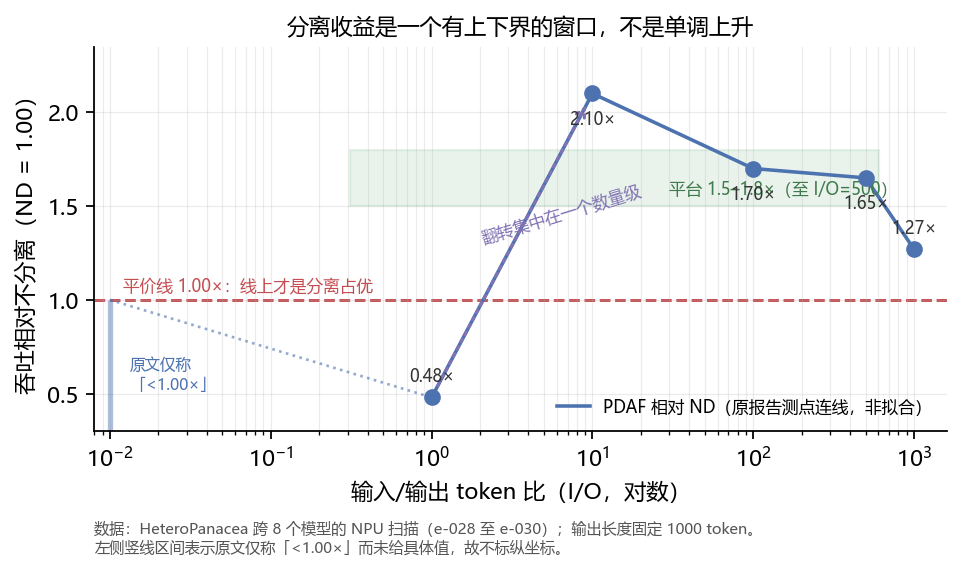
\includegraphics[width=\columnwidth]{figures/fig3_benefit_window.png}
\caption{分离收益随输入输出比的变化是一个窗口，不是单调上升。
数据取自 HeteroPanacea 跨 8 个模型的扫描（e-028 至 e-030）：
$I/O=1$ 时 $0.48\times$、$I/O=10$ 时 $2.10\times$、
平台期 $1.5$--$1.8\times$、$I/O=1000$ 回落至 $1.27\times$。
注：原作者只报了这几个离散点与区间，中间曲线为线性连接，
不是拟合结果。}
\label{fig:window}
\end{figure}

\subsection{按注意力结构的做法}

\noindent\textbf{MLA 系（DeepSeek-V3/V4 等）。} KV 极小，传输成本低，
故分离的门槛低、同机分离几乎白赚。但要注意一处反向效应：
\textbf{正因为 KV 小，分离的收益也随之变小}——收益侧来自两阶段
配置差异，而 KV 小意味着 decode 的带宽压力相对轻，两阶段的最优
配置被拉近。所以 MLA 模型「容易分离成功」与「分离收益大」
是两件事，不要混为一谈。

\noindent\textbf{GQA 系（Llama、Qwen 等）。} 处在中间。KV 比 MLA 大，
但又比 MHA 小得多，故传输成本可控而收益侧仍然明显。这一类的实测
材料最多：

\begin{itemize}
\item Qwen3-32B 在 8K 上下文下 KV 状态已达 \textbf{GB 级}；
  即便走 100\,Gbps 的 RDMA 网络，单次 post-prefill 传输也要
  \textbf{数百毫秒}，与 prefill 本身相当\texttt{[c-transfer]}。
  这个数字很关键：它说明「传输耗时」不能只按 250\,MB 的
  DeepSeek-V3 去估——换一个模型、换一个上下文长度，
  同一个耗时量级的结论会完全反过来。
\item Llama2-7B 上的系统性评测报告了阶段依赖的性能不对称：
  GPU 达成\textbf{低 $39\times$ 的延迟、高 $41\times$ 的吞吐}
  \texttt{[c-model]}。这是「两阶段画像相反」最直接的量化。
\item Llama 3.3 70B 在 $16\times$H100 集群上，分离方案在满足
  TTFT/TPOT SLO 的同时把\textbf{prefill 能耗降 39\%、
  decode 能耗降 48\%}\texttt{[c-model]}。能耗是常被忽略的一维，
  且两阶段降幅不同，正好对应配置差异。
\item Llama-13B 上，固定 prefill 长度 2048、把解码长度从 128 加到
  1024，\textbf{最大边际收益所在的阶段会移动}\texttt{[c-model]}。
  这直接说明「某模型的最佳配置」会随负载漂移。
\end{itemize}

\noindent\textbf{MHA 系。} KV 最大，传输成本最高。这一类在文献里
反而少见——因为分离对它最不划算，很少有人把它作为主实验对象。
这个\textbf{沉默本身就是证据}：把 MHA 模型放进分离框架，
要先算清 250\,MB 这个数字在它身上会放大几倍。

\subsection{按 FFN 结构的做法}

\noindent\textbf{MoE 系。} 多一层专家并行的复杂度。ExpertPlex 报告，
专家共享消除了超过 95\% 的重复模型权重，同时按需复用动态稀疏计算，
而注意力分离降低了注意力的通信开销\texttt{[c-model]}。
这说明 MoE 场景下的分离不只是 P/D 两分，还要考虑专家在两侧的放置。

\noindent\textbf{更细的分法：四路。} 如果把 FFN 也拆出来，
就得到四段（prefill-attention、prefill-FFN、decode-attention、
decode-FFN）。跨 8 个模型的比较显示，\textbf{四路 PDAF 是跨模型
最一致的做法}，在 8 个模型中的 6 个上是最佳模式，对 Llama-4
Maverick 与 Scout 分别达 $1.81\times$ 与 $1.77\times$
\texttt{[c-model]}。相比之下，只拆注意力与 FFN（AF）在所有测试
比例上都是最弱的，从未超过 ND，$I/O=100$ 时也只在
$0.20$--$0.65\times$\texttt{[c-boundary]}。

这个对比有方法论价值：\textbf{「拆得更细」不等于「更好」}。
AF 只拆一部分、且把两个阶段混在一起，结果最差；PDAF 拆得彻底，
结果最好。关键不是拆分粒度，而是\textbf{是否让每个子阶段独立配置}。

\subsection{按部署形态的做法}

\noindent\textbf{稀疏注意力 + CXL。} SAC 在 DeepSeek-V3.2 上用 SGLang
评测，相对 RDMA 基线取得 $2.1\times$ 吞吐、$9.7\times$ 更低的 TTFT、
$1.8\times$ 更低的 TBT\texttt{[c-model]}。含义是：当注意力本身变稀疏，
瓶颈转移到「\textbf{KV 放哪里}」而非「算得多快」，
此时载体的选择（CXL vs RDMA）比分离本身更重要。

\noindent\textbf{异构加速器。} HMA-Serve 在四块 Tenstorrent Blackhole
p150b（prefill）与一块 A100 80\,GB（decode）上实现，
经 100\,Gbps RDMA 互联\texttt{[c-transfer]}。这是把「两阶段画像不同」
推到极致的做法：不只换配置，直接换硬件类型。

\noindent\textbf{多模态：三段。} 唯一需要把分离从两段变三段的情形。
EAServe 指出，静态 50/50 切分虽然优于不切分，但仍然浪费了本地
prefill 容量\texttt{[c-model]}。原因是多模态多一个 Encode 阶段
（视觉编码），其资源画像又不同于 prefill 与 decode，
故 SGLang 提供 EPD（Encode-Prefill-Decode）三段分离。

\noindent\textbf{长上下文与容量。} LoongServe 指出，上下文窗口在快速
增长，导致资源使用的巨大方差，显存消耗随上下文线性上涨
\texttt{[c-model]}。这类场景下 KV 不只是传输成本问题，
还是\textbf{放不放得下}问题——分离顺带解决了容量，
故即使传输不便宜也可能划算。

\noindent\textbf{干扰而非带宽。} 一个容易忽略的失效模式：DeepSeek-V3.2
在 $DP=16$ 时，单条 prefill 请求可以拖住所有其它 decode 批次，
造成 \textbf{36.21\%--59.98\% 的空转率}\texttt{[c-model]}。
这里的瓶颈不是带宽也不是算力，而是调度干扰。
分离之所以有效，有一部分来自把这种干扰从架构上消除。

\subsection{跨模型的通用手段：逐阶段量化}

一个不依赖模型类型的做法：既然两阶段偏好不同，连量化精度也可以不同。
代价不对称——在 prefill 密集型任务上，只对 prefill 量化所付出的
精度损失，是只对 decode 量化的 $1.1$ 至 $4.1$ 倍（八个模型里
七个如此）\texttt{[c-model]}。故「按阶段分别量化」不是免费的，
prefill 侧对精度更敏感。

另一个例子来自格式分离：在 NVFP4 下，prefill 侧获得
$1.49\times$ 与 $1.67\times$ 相对 BF16 的加速，
而长上下文（$>$16K）时卸载使 NVFP4 prefill 延迟仅增加
不到 5\%（Qwen3）与 8\%（Gemma3）\texttt{[c-model]}。
后一个数字说明：\textbf{长上下文下卸载的代价比预期低}，
这与「长上下文必然传输昂贵」的直觉相反——因为卸载的是冷块。

\begin{table}[t]
\centering
\caption{决定分离做法的六个变量，只有前两个是模型属性。「轴」一列标出该变量影响的是传输成本侧还是并行策略侧——这是本文区分注意力轴与 FFN 轴的依据。}
\label{tab:model-vars}
\small
\begin{tabular}{@{}p{1.55cm}p{0.85cm}p{2.35cm}p{1.55cm}@{}}
\toprule
变量 & 轴 & 影响 & 是否模型属性 \\
\midrule
KV 每 token 大小 & 注意力 & MLA $<$ GQA $<$ MHA，差一个量级 & 是 \\
FFN 结构 & FFN & dense vs MoE，决定专家放置 & 是 \\
上下文长度 & --- & 线性放大 KV，兼有容量问题 & 否（业务） \\
输入输出比 & --- & 决定 P:D 配比，且收益有窗口 & 否（业务） \\
互联拓扑 & 成本 & 决定传输带宽档位 & 否（部署） \\
SLO & --- & 决定 goodput 定义与最优配比 & 否（业务） \\
\bottomrule
\end{tabular}
\end{table}

\subsection{为什么仍然不存在统一配置}

把上面合起来：最优做法取决于 KV 大小（注意力轴）× FFN 结构（并行轴）
× 上下文长度（业务）× 输入输出比（业务）× 互联拓扑（部署）×
SLO（业务）。六个变量里只有前两个是模型属性。

更关键的是，本轮新增的证据表明\textbf{收益随负载是窗口而非单调}，
且翻转集中在一个数量级内。这意味着：即使模型固定，
换一个业务负载就可能从 $2.10\times$ 掉到 $0.48\times$。

因此「某模型的最佳 PD 配置」这个提法缺的不只是自变量的个数，
还缺\textbf{适用区间}。可迁移的只能是判据：
在给定这六个变量的取值下，用第 \ref{sec:boundary} 节的条件判断
是否分离、按什么比例分离。

%% ===== sec8_technique.tex =====
\section{优化技巧：按作用对象分四类}
\label{sec:technique}

前一节讲的是「分不分、怎么分」。但一个已经上了分离的部署，
真正决定它跑得好不好的往往不是架构，而是\textbf{一串具体技巧}。
本节把这些技巧组织起来。

组织的维度不是「属于哪个框架」，也不是「新不新」，而是
\textbf{作用于哪个环节}。按此分四类\texttt{[c-technique]}：

\begin{table}[t]
\centering
\caption{优化技巧按作用对象分四类。同类的技巧互相替代，
异类可以叠加——故取舍问题不是「选哪个」，而是「每类选一个」。}
\label{tab:technique}
\small
\begin{tabular}{@{}p{1.15cm}p{2.0cm}p{2.5cm}p{1.3cm}@{}}
\toprule
类别 & 作用于 & 代表技巧 & 实测幅度 \\
\midrule
A 省传输量 & KV 字节数本身 & 逐层传输、chunk 级传输、
  KV 压缩/量化、前缀缓存 & 成比例 \\
B 让传输不可见 & 传输与计算的时序 & TBO、SBO、DBO、piggyback
  & 隐藏传输 \\
C 均衡负载 & 每个 rank 分到多少 & Waterfill、LPLB、EPLB、
  请求迁移、弹性配比 & 0.84--7.34\% \\
D 省 decode 步 & 要跑多少步 & DSpark 自适应验证、投机解码
  & 前沿 \\
\bottomrule
\end{tabular}
\end{table}

四类的性质完全不同，混着谈会得出错误结论。以下逐类说。

\subsection{A 类：省传输量}

最直接的一类——传输成本与字节数成正比，那就少传。

\noindent\textbf{逐层传输。} 不等整个 prefill 算完再传，而是每算完
一层就异步传该层的 KV，prompt 计算同时进入下一层。Splitwise 的做法是：
在每层末尾触发该层 KV 的异步传输，让 prompt 计算继续
\texttt{[c-technique]}。好处有三——传输被计算掩盖、token 阶段可以
更早开始、prompt 机器可以更早释放显存。

\noindent 但这条技巧\textbf{有适用下限}，这点常被忽略：原文明确指出，
小 prompt 时 KV 很小，「没有必要为逐层传输所需的细粒度同步付出开销」
\texttt{[c-technique]}。也就是说，逐层传输把一次大传输切成 $L$ 次
小传输，每次都付固定开销；当 KV 总量小到固定开销占比显著时，
切得越细越亏。

\noindent\textbf{chunk 级传输。} 与逐层同类但切分维度不同：沿
chunked prefill 的 chunk 切，使 prefill 与 KV 传输并行。
另有 request 级传输，用来减少传输次数（一次传整个请求的 KV）。
原文把三者的关系说清了：chunk 级让计算与网络并行，request 级
最小化传输次数，逐层则可与 chunk 级结合以进一步并行
\texttt{[c-technique]}。

\noindent 这三者是同一维度的不同粒度。选哪个取决于两件事：
固定开销占多大（粒度太细不划算）、以及 prefill chunk 有多长
（chunk 级需要 chunked prefill 才有意义）。

\noindent\textbf{KV 压缩与量化。} 直接从字节数下手。第
\ref{sec:model} 节已提到逐阶段量化的代价不对称：只量化 prefill 的
精度损失是只量化 decode 的 $1.1$ 至 $4.1$ 倍\texttt{[c-model]}。
所以压缩要用在 decode 侧更划算——那里 KV 读得多、且对精度更宽容。

\noindent\textbf{前缀缓存。} 相同前缀不重算、也不重传。
严格说它省的是 prefill 计算而非传输，但它会\textbf{改变传输量的分布}：
命中前缀后需要搬的 KV 变小，于是前面所有按「全量 KV」算的成本估计
都要下调。这是部署时最容易低估的一条。

\noindent\textbf{重算 vs 传输。} 还有一个非技巧的技巧：KV 太小时，
\textbf{重算比传输便宜}。这条与第 \ref{sec:boundary} 节的
「上下文极短导致固定开销主导」是同一件事的两面。

\subsection{B 类：让传输不可见}

不减少字节数，而是让传输发生在计算的同时，从而在端到端时间里
看不见它。这一类全部依赖\textbf{MoE 的 all-to-all 通信}与
\textbf{attention 计算}可以交错这一事实。

\noindent\textbf{TBO（Two-Batch Overlap）。} 把请求拆成两个
micro-batch，让一个 micro-batch 的 attention 计算与另一个的
dispatch/combine 通信交错。SGLang 的官方描述是：TBO 把请求拆成
micro-batch，把 attention 计算与 dispatch/combine 操作交错，
执行图中的 yield 点允许暂停以形成重叠，从而在\textbf{不增加峰值显存}
的前提下提高吞吐\texttt{[c-technique]}。

\noindent 最后半句是关键：TBO 不靠加显存换吞吐，靠的是给通信
找一个可以并行的伙伴。

\noindent\textbf{SBO（Single-Batch Overlap）。} 不拆 batch，
而是在同一个 micro-batch 内部把通信与 shared expert 的计算重叠
\texttt{[c-technique]}。相比 TBO，SBO 不需要拆 batch，
故没有「拆完每半太小、GEMM 效率下降」的风险，但可重叠的窗口也更窄
（只有 shared expert 那一段）。

\noindent\textbf{DBO（Dual Batch Overlap）。} vLLM 的实现思路相同但
手段不同：在 model runner 里把 batch 拆成两个 micro-batch，
\textbf{起两个 worker 线程}各跑一半，在两个线程之间设置 yield 点，
使一个在算时另一个在等通信，形成乒乓\texttt{[c-technique]}。

\noindent DBO 有一段值得记的工程细节：拆不拆要\textbf{跨所有 DP rank
统一决定}——只要有一个 rank 拆不动，全体都不拆；且若 padding 后
某个 rank 的第二个 micro-batch 为空，也全体放弃\texttt{[c-technique]}。
这是「并行组内必须同步决策」的典型代价。

\noindent 更实用的是它的\textbf{阈值}：DBO 只在 batch 的 token 数超过
阈值时才启用，低于阈值不拆\texttt{[c-technique]}。原因不难推：
拆成两半后每半的 GEMM 变窄、线程切换有成本，小 batch 上得不偿失。

\noindent\textbf{piggyback。} 让 decode 搭 prefill 的便车一起批处理
（Sarathi-Serve 的做法：把 decode 挂到 chunked prefill 上）。
它在不分离的架构里替代分离——这一点很重要：
\textbf{B 类技巧里有几个是分离的替代品，不是补充}。

\noindent 这一类的共同前提是 \textbf{MoE + EP}。若模型是 dense，
没有 all-to-all 可重叠，B 类基本失效。这是选型时第一个要看的。

\subsection{C 类：均衡负载}

MoE 的 router 不产生均匀的专家流量，某些专家收到的 token 远多于
其它，EP 组于是等最忙的那个 rank。C 类技巧处理这件事。

\noindent\textbf{Waterfill。} 一个轻量的 shared-expert 负载均衡：
把 shared expert 通过 DeepEP 派发，并\textbf{指派给负载较轻的 rank}
\texttt{[c-technique]}。实测：在两台 Hopper 节点上跑 DeepSeek-V3/R1
风格负载，Waterfill 在 MMLU、GPQA、GSM8K 上把总吞吐提升
\textbf{+1.48\% 至 +4.66\%}；在 DeepSeek V4 上最好测点从
49{,}253\,tok/s 提到 51{,}677\,tok/s（+4.92\%）\texttt{[c-technique]}。

\noindent 注意幅度：个位数百分比。这类技巧\textbf{不是数量级的改进}，
但它的成本也很低（只改派发目标，不动权重、不改路由）。

\noindent\textbf{LPLB。} 针对\textbf{冗余专家副本}的线性规划均衡器：
对每层解一个 dispatch 优化问题，在冗余副本之间重新分配 token
\texttt{[c-technique]}。实测：同样的两台 Hopper 节点、同样的
冗余 EPLB 放置，LPLB 把总吞吐提升 \textbf{+0.84\% 至 +7.34\%}
\texttt{[c-technique]}。

\noindent LPLB 有一个必须说清的性质：它\textbf{不移动权重，也不改变
router 的逻辑决策}，只改物理副本的分配\texttt{[c-technique]}。
故它不损精度——这一点与量化类技巧形成对比，也是它能「默认打开」
的原因。

\noindent\textbf{两个前置依赖，缺了就只有开销。}

第一，\textbf{必须有冗余副本}。原文明确：在 \texttt{red0}
（无冗余副本）配置下，没有副本可重新平衡，算法无法改善派发，
其 all-reduce 与求解路径\textbf{纯粹表现为开销}\texttt{[c-technique]}。

第二，\textbf{收益取决于在线流量的分布与标定分布的偏离程度}。
原文的说法是 LPLB 的收益「跟随 live batch 偏离标定分布的程度」，
并在中等规模处最强\texttt{[c-technique]}。

\noindent 这两条合起来说明一件事：C 类技巧的收益是
\textbf{有条件的、个位数百分比},不该被当成「开了就变快」的开关。

\noindent\textbf{PD 给 C 类带来的新约束。} 这是本节最需要单独讲的
一处交互。DP attention 下，\textbf{不同的 EP rank 在同一步跑不同的
forward 模式}——有的在跑 prefill、有的在跑 decode、有的 idle。
于是没有单个 rank 能看到全局的 token 分布\texttt{[c-technique]}。

\noindent 后果很具体：均衡算法的输入（全局各专家的 token 计数）
在 PD 下不是本地可得的，必须额外做一次 all-reduce 才能拼出来。
这既是开销，也是延迟——负载均衡决策要等全局信息到齐。

\noindent 这一条解释了为什么有些在不分离部署里跑得很好的均衡技巧，
搬到 PD 上收益变薄：\textbf{信息可见性被架构改变了}。

\noindent\textbf{其它 C 类手段。} EPLB（静态专家放置）、
请求迁移（Llumnix 在运行时重调度请求）、以及弹性配比
（FluidPD 在运行时改 P:D 比）。它们作用于不同的时间尺度：
EPLB 是天级、请求迁移是秒级、弹性配比是分钟级。
\textbf{不同时间尺度的手段可以叠加}，因为它们不抢同一个决策点。

\subsection{D 类：省 decode 步}

decode 的每一步都要读全部权重与 KV，故减少步数是最直接的加速。
投机解码就是这条路：用小模型起草 $k$ 个 token，大模型一次验证。

\noindent 但这条路有一个\textbf{随负载反转}的收益结构。原文说得很清楚：
batch size 为 1 时这是笔好交易——GPU 受显存带宽限制、算力有余，
起草的额外计算近乎免费；到 batch size 256 时这笔交易就微妙了，
draft token 开始与真 token 抢同一份算力，每个被拒的 token 都浪费
了有用的算力，被拒够多时吞吐显著下降\texttt{[c-technique]}。

\noindent 为什么会拒？因为\textbf{逐位置存活率衰减很快}：在
DeepSeek-V4-Pro-0813 上，一个 7 token 块的最后一个 token 存活率
不足 10\%，而第一个超过 70\%\texttt{[c-technique]}。那个低概率的
token 在每次验证批里都占一个槽位——显存受限时这个槽位是免费的，
算力饱和后它就有真实成本。

\noindent\textbf{DSpark 的做法}：给每个 draft token 打一个置信度，
\textbf{按步决定验证多少}，而不是按部署选一个固定的
\texttt{num\_speculative\_tokens}\texttt{[c-technique]}。

\noindent 效果：开启自适应验证后，投机解码在并发 1 到 256 全程都能
带来收益，且低并发时仍保有长 draft 的好处\texttt{[c-technique]}。
原文的说法是「停留在 Pareto 前沿的边缘」\texttt{[c-technique]}。

\noindent 这条技巧的意义超出它自身：它是\textbf{把静态超参换成按负载
决策}的一个范例。前面 A、B、C 三类里的阈值（DBO 的 token 阈值、
LPLB 的冗余度）都可以用同样的思路做成自适应。

\noindent\textbf{代价与限制。} DSpark 需要 ALWAYS 级的 CUDA graph
支持，故不支持 \texttt{--enforce-eager}、LoRA 与 pipeline
parallel\texttt{[c-technique]}。这是 B、D 两类共有的特征：
\textbf{越依赖 kernel 级重叠的技巧，对执行模式的要求越硬}。

\subsection{补充三类：数据通路、准入、并行度重切分}

上面四类是按「作用于哪个环节」分的。还有三类技巧不落在这四类里，
但都是 PD 部署上实际在用的，且各有独立的量级。

\noindent\textbf{\sym{①} 数据通路层：不是少传，而是让每次传输更便宜。}

最典型的是 \textbf{zero-copy}：让发送/接收 kernel 直接操作应用的数据区，
省掉中间那一次拷贝\texttt{[c-technique]}。在 CloudMatrix384 的
send/recv 设计里，除了基于内存语义（MTE2/MTE3）的传输路径，
还专门提供 zero-copy 版本\texttt{[c-technique]}。

\noindent 与之配套的是 \textbf{GPUDirect RDMA}：让网卡直接读写显存，
绕过主机内存。Mooncake 把 KV 块在 CPU 与 GPU 之间的搬移交给一个
独立的 GPUDirect RDMA 组件（Messenger）\texttt{[c-technique]}。

\noindent 这一类的收益不在「传得少」，而在\textbf{把传输从「要经过
CPU 与两次拷贝」变成「网卡直接进显存」}。它与 A 类正交，可以叠加。

\noindent\textbf{\sym{②} 准入与拒绝：容量不够时不排队，直接拒。}

这条在过载场景下最重要，也最常被忽略。传统研究假设所有请求都会被处理，
但真实的高负载场景下，\textbf{把注定超时的请求排进队列只会拖垮其它请求}。

\noindent Mooncake 的做法是\textbf{预测式 early rejection}：先预测这条
请求能否在 SLO 内完成，不能就早拒\texttt{[c-technique]}。效果：在
某些模拟场景下吞吐最高提升 \textbf{525\%} 且仍满足 SLO；在真实负载下
让 Kimi 多处理 \textbf{75\%} 的请求\texttt{[c-technique]}。

\noindent 这是本文所引技巧里\textbf{幅度最大的一条}，但它提升的不是
「单位时间算得更多」，而是「单位时间算的都是有用的」。二者在过载时
差别巨大。

\noindent 这也解释了为什么它属于 PD 的优化技巧：分离之后 P 与 D 的
队列是独立的，一条请求要过两个池子，\textbf{任一池子超时都白做}，
故准入判断必须放在分离之前，且要同时考虑两段的排队时间。

\noindent\textbf{\sym{③} 并行度重切分：运行中改 DP/TP/PP 布局。}

比「弹性改 P:D 比」更激进的一层——不只改两阶段的比例，而是改
\textbf{每个阶段内部的并行方式}，并为此重新切分权重与重算 KV。

\noindent 有一个完整的实测：某系统以 Layout A 起步，当活跃轨迹数降到
批量的 10\% 以下时切到 Layout B（DP=8、PP=16、TP=8），
切换要付一次\textbf{权重 reshard 与 KV 重物化}的代价
\texttt{[c-technique]}。收益：rollout makespan 从 528.8\,s 降到
259.1\,s，有效 decode 吞吐提升 2.04 倍\texttt{[c-technique]}。

\noindent 原文把这归因为「相位匹配的并行度」：Layout A 吸收密集突发，
而重新切分让稀疏尾部的 decode 效率回升\texttt{[c-technique]}。

\noindent 这一类的取舍很清晰：\textbf{重切分有一次性成本，
故只在相位持续足够久时才划算}。这与第 \ref{sec:boundary} 节的
「窗口」是同一个道理——收益要摊得平固定成本。

\subsection{怎么选：三条判据}

把四类放在一起，取舍可以按三条判据走。

\noindent\textbf{\sym{①} 先看模型是不是 MoE + EP。} 若不是，B 类（TBO/SBO/
DBO）基本不可用，因为没有被重叠的 all-to-all。这一步就能砍掉一半选项。

\noindent\textbf{\sym{②} 每类选一个，先做前置条件检查。} 同类别替代，
故不必都上。但每条都有前置条件：逐层传输要求 KV 够大（否则固定开销
主导）；LPLB 要求有冗余副本（\texttt{red0} 下只有开销）；
DBO 要求 token 数过阈值；DSpark 要求 CUDA graph 全量模式。
\textbf{前置条件不满足时，开了是负收益}——这是本文最想强调的一点。

\noindent\textbf{\sym{③} 按幅度排优先级。} A 类与 C 类不在一个量级：
A 类按传输比例省（可能省掉一半），C 类是个位数百分比
（$0.84\%$--$7.34\%$）。D 类的幅度取决于并发——低并发时大、
高并发时靠自适应才不亏。

\noindent 所以合理的顺序是：\textbf{先用 A 类把量降下来，
再用 B 类把剩下的藏起来，然后用 D 类减少步数，
最后用 C 类抹平尾部不均}。反过来做（先上 C 类）会得到
「调了很久只有 3\%」的体验。

\noindent 最后一条经验值得单独记：\textbf{这四类里有几条是分离的替代品
而非补充}。piggyback（decode 搭 prefill 的便车）与 chunked prefill
在不分离架构里就能拿到相当一部分收益。若一个部署还没上分离，
先试 A 类与 piggyback 的性价比通常高于直接上分离——这与第
\ref{sec:boundary} 节的判据一致：分离是这些手段里最贵的一个。

%% ===== sec9_plane.tex =====
\section{四类之外：按实现平面重看优化栈}
\label{sec:plane}

第 \ref{sec:technique} 节的四类是按「作用于 KV 传输成本的哪个环节」
分的：省量、隐藏、均衡、少步。这个维度覆盖了\textbf{分离本身带来的
额外成本}，但它不是唯一的切法，也不覆盖全部优化。

对照生产系统的实际做法就能看出边界。vLLM 的大规模服务文档列出九项
关键优化，把每 H200 的吞吐从约 1{,}500 提到 2{,}200\,tok/s——其中
\textbf{六项与 KV 传输无关}\texttt{[c-plane]}：异步调度、CUDA graph 的
\texttt{FULL\_AND\_PIECEWISE} 模式、DeepGEMM、DeepEP kernel、
SiLU kernel、算子融合。

这说明四类不够。本节换一个维度重看：按\textbf{实现平面}分。

\subsection{三平面框架}

生产系统普遍把优化分成三个平面\texttt{[c-plane]}：

\begin{table}[t]
\centering
\caption{三平面与各自的优化手段。与第 \ref{sec:technique} 节的四类
正交——四类只回答「分离的那笔账怎么省」，三平面回答「整个栈有哪几层可以动」。}
\label{tab:plane}
\small
\begin{tabular}{@{}p{1.05cm}p{3.5cm}p{3.9cm}@{}}
\toprule
平面 & 管什么 & 代表手段 \\
\midrule
数据面 & KV 放哪、留多久 & KV 池分层、打包布局、
  session 感知保留、前缀缓存 \\
执行面 & 单步算多快 & 并行策略（DEP/DCP/PCP/Wide-EP）、
  kernel 融合、CUDA graph、异步调度 \\
控制面 & 谁在什么时候被调度 & 长 prefill token 上限、
  prefill 节拍、路由策略、准入、P/D 配比 \\
\bottomrule
\end{tabular}
\end{table}

\noindent 这个划分比四类更好用的地方在于：它对应\textbf{不同的负责人
与不同的时间尺度}。数据面是容量规划，执行面是 kernel 与并行团队，
控制面是调度策略。四类都在控制面与执行面的交界处，看不全。

\subsection{执行面：完全不涉及传输的优化}

这是四类漏得最多的一块。它不减少传输、也不隐藏传输，
而是\textbf{直接把单步算得更快}。

\noindent\textbf{算子融合。} 把多个小算子合成一个 kernel，省掉中间的
读写与启动开销。实测幅度不小：

\begin{itemize}[leftmargin=1.3em,itemsep=1pt,topsep=2pt]
  \item SiLU-mul-quant 融合、Cutlass QKV kernel 等改进，与 DBO 一起
        构成 1.5k$\to$2.2k\,tok/s/H200 的主要来源\texttt{[c-plane]}。
  \item Kimi K3 的 GEMM 与 reduce-scatter 融合，改善序列并行的通信
        \texttt{[c-plane]}；latent-tail MoE 融合把端到端延迟降约
        $5\%$\texttt{[c-plane]}。
  \item 用对称内存把 query 多播、部分输出与 LSE 直接写进对端接收槽，
        再在 kernel 内融合——每层延迟降约 $13\%$\texttt{[c-plane]}。
  \item MiniMax M3 的长上下文 indexer（CuteDSL），GB300 上延迟改善
        约 $3\%$ 至 $31\%$，取决于 shape\texttt{[c-plane]}。
\end{itemize}

\noindent 这些数字有个共同特征：\textbf{个位数到三十个百分点，
但都是端到端可见的}。它们不依赖架构选择，改动局部，
是投入产出比最高的一类——也正因如此，它们最容易被
「这是 kernel 团队的事」推给别人，然后从架构讨论里消失。

\noindent\textbf{并行策略：不是「均衡」，是「选哪种切法」。}

我在四类里把负载均衡与并行放在一起谈，这是不准确的。并行策略
是\textbf{选切分维度}，与均衡是两个问题。

\noindent 同样的模型，不同切法的差别是数量级的：
DeepSeek V4 在 32K prompt 上，prefill 上下文并行（PCP8）相对张量并行
（TP8）有 $2.65\times$ 的 prefill 加速\texttt{[c-plane]}。Kimi K3 的
decode 上下文并行（DCP）沿序列切 KV，每个 rank 只留 $1/N$ 的状态，
既降 decode 延迟又扩大 KV 容量\texttt{[c-plane]}。

\noindent 但\textbf{切法必须服从模型架构}，这是本节最重要的一条，
而它是从一个反例得出的。DeepSeek V4 的压缩稀疏注意力包含 indexer、
compressor 与主注意力三部分，上下文并行必须切分并协调全部子层。
vLLM 团队「在重叠通信与优化对应 kernel 上投入很大」，最后
DCP \textbf{只是打平 DEP，没有超过}\texttt{[c-plane]}。

\noindent 原文的总结值得直接引：\textbf{并行必须跟随模型架构；
在一个隐注意力模型上成功的策略，未必能推广到另一个}
\texttt{[c-plane]}。这解释了为什么第 \ref{sec:model} 节按模型给做法
是对的——但理由不是「模型大小不同」，而是\textbf{注意力结构的内部
组成不同，可切的维度就不同}。

\noindent\textbf{第二个反例：流水线并行不适合热轮次。} PP（含 chunked PP）
在长而新的 prompt 上表现很好——大 prefill 提供的计算足以填满各级流水线，
吞吐近线性扩展。但 agentic 场景的多数轮次已有系统提示与前几轮缓存，
每个新请求只增加几百到几千 token，\textbf{没有足够的新计算填满流水线，
bubble 吃掉大部分潜在收益}\texttt{[c-plane]}。

\noindent 原文的措辞很克制：「教训不是 PP 无效，而是它对冷的、
计算重的 prefill 有效，但不该成为热的、前缀重的轮次的默认」
\texttt{[c-plane]}。这是一条\textbf{按负载形态选并行}的判据，
比任何「PP 好/不好」的结论都有用。

\subsection{数据面：容量与命中率}

四类里的 A 类（省传输量）只管「少搬」，但生产系统还有另一半：
\textbf{把 KV 留在更近的地方，提高命中}。

\noindent\textbf{KV 池分层。} 把分布式 KV 池做成多层，用磁盘与纯 CPU
节点扩容量；\texttt{standalone-store} 模式下由外部 Mooncake 客户端
持有 CPU 池与磁盘层，vLLM worker 变成纯请求方\texttt{[c-plane]}。

\noindent\textbf{打包布局。} 这个细节很能说明问题：DeepSeek V4 早期的
KV 布局把不同 cache 类型碎成三个尺寸桶、分配了 \textbf{92 个独立
tensor}，padding 浪费显存，且对 P/D 传输与 offload 都不友好。
新的打包布局把全部 cache group 与层放进每块一个连续分配
\texttt{[c-plane]}，减少描述符与 P/D 传输开销，并允许更小的分配单元
（开 FP4 indexer 时省约 $10\%$ 的 KV 显存）\texttt{[c-plane]}。

\noindent 这一条对本文主题有直接含义：\textbf{数据传输效率不只取决于
网络，还取决于内存布局}。同样的字节数，碎片化布局要发 92 个描述符，
打包布局只发一个。这属于「让传输便宜」，但既不在我的 A 类
（省量）也不在 B 类（隐藏）里。

\noindent\textbf{session 感知的保留。} 对混合了线性/滑窗注意力与全注意力
的模型，前缀复用需要在复用边界上保留线性状态或滑窗缓存。
逐 token 保存太贵，故两条策略并用：按间隔保留每轮 prompt 末尾的状态；
以及「同一前缀被观察到第二次时才保留检查点」\texttt{[c-plane]}。

\noindent 这条的判据是\textbf{观测到第二次才投资}——把存储成本
押在有复用证据的前缀上，而不是预测哪些前缀会被复用。

\subsection{控制面：调度顺序与路由}

\noindent\textbf{调度顺序：一个被四类完全漏掉的维度。}

我原来的 B 类是「让传输不可见」，讲的是 micro-batch 交错。
但控制面还有另一个问题：\textbf{队列里的顺序}。

\noindent vLLM 的 chunked-prefill 调度器默认先进先出。一条长 prefill
会一步接一步地占满整个 token 预算，同 rank 上排队的短轮次
\textbf{在长 prefill 结束前完全无法被调度}——这就是队头阻塞。

\noindent 修法是给单条请求每步可调度的 token 数设上限
（\texttt{--long-prefill-token-threshold}）。用 512 token 的阈值，
长 prefill 就给短轮次留出空间，让它们同批加入、更早开始 decode。
在 B300 上跑 DeepSeek V4 Pro，这使每 GPU 每秒总 token 数（TPGS）
提升最多 $93\%$，P90 交互性约 $2.3\times$\texttt{[c-plane]}。

\noindent 代价也写清了：长请求自身的 TTFT 变高，故对 TTFT 敏感
的部署要用更大的阈值\texttt{[c-plane]}。

\noindent 幅度上，这条比四类里任何一条都大——$93\%$ 与 $2.3\times$，
而 C 类均衡是个位数百分比。原因不难理解：队头阻塞\textbf{让整个
队列白等}，而均衡只抹平尾部差距。

\noindent 还有一条更细的：DEP 下 MoE 的 all-to-all 迫使各 rank 同步推进，
一个 rank 在处理 prefill 就拖慢整组。若 prefill 在各 rank 的不同步
到达，这个代价被反复支付。修法是设 \texttt{--prefill-schedule-interval}，
只每隔 $N$ 个引擎步接纳 prefill，把 prefill 集中到相同的步上，
使其余步成为纯 decode\texttt{[c-plane]}。

\noindent\textbf{路由：一个必须写进正文的反例。}

\noindent 四类的 C 类假设均衡有价值。生产实测推翻了它。

\noindent 观察到聚合部署里各 rank 的 KV 使用严重不均，自然的反应是按
队列深度、运行 token 数或当前 KV 利用率来均衡请求。
\textbf{但这些策略全部劣于简单的 session 粘性路由}\texttt{[c-plane]}。

\noindent 机制值得逐字理解：agentic 会话的轮次间隔很短，下一轮到达时
它的前缀往往还在上一张卡上。把会话迁到更空的 rank，就必须去取 KV——
即使前缀保存在分布式池里。传输是异步的、与计算重叠的，
\textbf{但它不是免费的}：预取的块会临时占用目标 rank 的 GPU KV 容量，
减少它能接纳的序列数。结果是\textbf{队列更均衡了，总并发却更少}
\texttt{[c-plane]}。

\noindent 原文的结论是：轮次间隔短时，\textbf{保住会话局部性比完美
均衡瞬时负载更有价值}；路由必须考虑每个 worker 上已驻留的状态，
而不只是排队的量\texttt{[c-plane]}。

\noindent 这一条对本文的判据是一个补充而不是否定：第
\ref{sec:boundary} 节说分离要考虑负载是否落在窗口内，
现在要加一句——\textbf{即使落在窗口内，均衡策略也可能让收益变薄}，
因为均衡与局部性冲突。

\subsection{四类与三平面是什么关系}

写到这里可以说清两套划分的关系，这也是本节最想给出的结论：

\begin{itemize}[leftmargin=1.3em,itemsep=1.5pt,topsep=2pt]
  \item \textbf{四类是按成本链切的}，覆盖「KV 传输这笔账怎么省」。
        它的优点是能直接对应到收益与代价，缺点是看不到传输之外的层。
  \item \textbf{三平面是按实现层切的}，覆盖「整个栈有哪几层可以动」。
        它的优点是完备，缺点是不能直接告诉你「哪个划算」。
  \item \textbf{两者正交，应该叠加使用}：用三平面保证不漏，
        用四类判断传输那一层的取舍。
\end{itemize}

\noindent 若只能记一句，我选这一句：\textbf{四类解决的是分离引入的
额外成本；而生产系统里最大的单项收益往往来自与分离无关的执行面
改进}——$2.65\times$ 的 PCP、$93\%$ 的调度上限、$13\%$ 的 kernel 融合，
都不在四类里。把注意力全放在「怎么把 KV 搬得更快」，
会错过这些。

%% ===== sec6_boundary.tex =====
\section{收益的边界：什么时候不该分离}
\label{sec:boundary}

文献普遍报告正收益，但这里有一个发布偏差：失败的部署不会写成论文。
故本节的证据需要主动找——找那些\textbf{专门问「何时不划算」}的工作。

\subsection{一条直接的判据}

最清晰的表述来自对 Prefill--Decode--Attention--FFN 四段分离的模拟研究：
更细的分离粒度「不保证值得它的复杂度」，收益取决于模型架构，
也取决于负载的 prefill/output 比率\texttt{[c-boundary]}。

这句话的价值在于它把问题从「分离好不好」改成了
「在当前架构与负载比下，分离好不好」。前者无解，后者可测。

\subsection{收益是一个窗口，不是一个倍数}

上一句还只是说「取决于比率」。本轮的证据把它量化了，而且结论比
「取决于」更强：它是一个\textbf{有上下界的窗口}，且\textbf{非单调}。

同一项研究跨 8 个模型、扫 9 个输入输出比，报告了三段结果
（第 \ref{sec:model} 节已述，此处只说边界含义）：

\begin{itemize}
\item 在 $I/O = 0.01$ 与 $I/O = 1$ 时，不分离对\textbf{每一个}被测模型
  都是最强配置，PD、AF、PDAF 全线低于 $1.00\times$
  \texttt{[c-window]}。这不是「模型选错了」，是负载没到那个区间。
\item 在 $I/O = 100$ 时，PDAF 对全部 8 个模型超过不分离
  （$1.05$--$1.92\times$），PD 对 8 个中的 7 个超过
  \texttt{[c-window]}。仍然有例外：DeepSeek-V4-Pro 在 $0.95\times$。
\item 翻转集中在\textbf{一个数量级}之内：$I/O=1$ 时 $0.48\times$，
  $I/O=10$ 时已是 $2.10\times$；此后平台化在 $1.5$--$1.8\times$
  至 $I/O=500$，到 $I/O=1000$ \textbf{反而回落到 $1.27\times$}
  \texttt{[c-window]}。
\end{itemize}

第三条是本节最需要记住的：\textbf{收益有上界}。当 prefill 大到成为
系统瓶颈后，为 decode 单独配置的硬件开始空闲——分离的成本从「传输」
变成了「闲置」。此前讨论分离的文献几乎只谈下界（负载太轻不划算），
没有谈上界。

因此本文第 \ref{sec:model} 节的判据第三条要改写：不是「负载足够重」，
而是「\textbf{负载落在窗口内}」——太轻与太重都不划算。

这是一个可操作的差别：只判断「够不够重」会让人在最重的工作负载上
做分离，而那恰好是收益回落的区间。

\subsection{四类使分离失效的条件}

\noindent\textbf{\sym{①} 传输成本超过收益。} 这是最直接的一类。由第
\ref{sec:transfer} 节的数据，同一份 250\,MB 的 KV 经 RDMA 传输需 10\,ms。
若 decode 的单步时延目标是 50\,ms 量级，传输就吃掉了 20\%——
而分离带来的配置优化能否补回这 20\%，要看收益侧有多大。

但要注意这个数字不能随便外推：Qwen3-32B 在 8K 上下文下 KV 已达
GB 级，走 100\,Gbps RDMA 时单次传输需\textbf{数百毫秒}，
与 prefill 本身相当\texttt{[c-transfer]}。同一个「传输耗时」
在不同模型与上下文长度下能差一个数量级以上。

\noindent\textbf{\sym{②} 两阶段资源画像接近。} 小模型、短上下文、单卡可容纳
全部权重与 KV 时，prefill 与 decode 的最优配置差别很小。此时分离只增加
传输与复杂度，收益趋近于零。

\noindent\textbf{\sym{③} 负载本身很轻。} 算力闲置时，配置是否最优无关紧要——
反正都够快。分离的收益本质上来自「在资源紧张时把资源用得更对」，
资源不紧张时这个收益无从兑现。这一条现在有了定量支撑：
$I/O \le 1$ 时 8 个模型全部不支持分离\texttt{[c-boundary]}。

\noindent\textbf{\sym{④} 上下文极短导致固定开销主导。} 这一条最反直觉：
KV 绝对量小时，按字节数算传输应该很快，但建连、内存注册、同步这些
固定开销不随消息大小缩放。此时带宽不是瓶颈，固定开销才是。

\noindent\textbf{\sym{⑤} 干扰没有被消除。} 还有一类失效容易被漏掉：瓶颈既不是
带宽也不是算力，而是调度干扰。DeepSeek-V3.2 在 $DP=16$ 时，
单条 prefill 请求可以拖住所有其它 decode 批次，造成
$36.21\%$--$59.98\%$ 的空转率\texttt{[c-model]}。这种情况下分离的价值
主要来自从架构上消除干扰，而非带宽；反过来，如果部署的调度器已经能
隔离干扰，分离的收益就要打折扣。

\subsection{一个明确的反例}

必须单独列出这条，因为它直接挑战「分离更优」的默认假设。

有工作报告：相对 PD 分离与 PD 聚合，某方案的 TTFT 最多降低 13.2×，
TPOT 最多降低 1.69×\texttt{[c-boundary]}。也就是说，
\textbf{存在一种方案，在 TTFT 上比分离好 13 倍}。
如果只读「分离 vs 不分离」的对比，会完全看不到这个量级的改进空间——
因为分离本身可能不是这个维度上的最优解。

这条证据的意义不在于否定分离，而在于提醒：
「分离 vs 混部」是一个二选一的问题框架，而真实的设计空间里
还有第三、第四种做法（如按注意力与 FFN 再拆、如用 CXL 换载体）。
把问题设成二选一，会系统性地漏掉这些。

\subsection{判据汇总}

\begin{table}[t]
\centering
\caption{分离的决策判据。四项全满足才建议分离；任一项不满足时，应优先考虑 chunked prefill
等零传输成本的方案。第三条由 HeteroPanacea 的 8 模型扫描定量支撑（e-028 至 e-030）。}
\label{tab:criteria}
\small
\begin{tabular}{@{}p{0.35cm}p{3.0cm}p{2.5cm}@{}}
\toprule
\# & 条件 & 检查方式 \\
\midrule
1 & 两阶段最优配置显著不同 & 分别做单阶段压测，比最优并行度与 batch \\
2 & 存在高带宽 KV 通路 & 同机 NVLink 或跨机 RDMA，而非共享存储 \\
3 & 负载落在窗口内 & 太轻不划算，太重则 decode 硬件闲置 \\
4 & KV 规模足够大 & 传输固定开销占比可忽略 \\
\bottomrule
\end{tabular}
\end{table}

这四项不是充分条件，但是必要条件——任一项不满足时，
分离的收益很难为正。它们也是可操作的：每一项都能在部署前测出来。

%% ===== sec7_discuss.tex =====
\section{讨论}
\label{sec:discuss}

\subsection{本文的结论有多可靠}

需要区分两类结论。

\textbf{第一类是量化的}：NVLink 与 RDMA 的传输耗时相差 16.7 倍、
聚合方案把 TTFT 降低 13.2 倍、专家共享消除 95\% 重复权重。
这些数字都能追到具体证据与原文（\texttt{analysis.json}），
但它们都是\textbf{别人在别人的条件下测的}。换硬件、换模型、换负载，
数值会变。故本文引用它们时始终带上条件，不给孤立数字。

\textbf{第二类是判据性的}：分离的净收益 ≈ 收益侧的配置优化
$-$ 成本侧的 KV 搬运。这个式子的形式是可辩护的（它只是收支相抵），
但本文\textbf{没有}给出各项的系数——那需要自己的实验。
故第 \ref{sec:boundary} 节的四项判据应被当作\textbf{检查清单}，
而不是可代入计算的模型。

\subsection{一个反复出现的模式}

整理这些材料时，一个模式反复出现：\textbf{几乎所有的收益都来自
「按阶段区分对待」，而不是来自「分离」这个具体手段}。

chunked prefill 区分了两阶段的时间片；分离区分了两阶段的硬件；
逐阶段量化区分了两阶段的精度；EPD 把区分扩展到三段。
它们的共同点是承认「prefill 与 decode 要的东西不同」，
而分离只是实现这个承认的一种方式——且是成本较高的一种
（要搬 KV、要多实例、故障域变大）。

这个视角解释了为什么 chunked prefill 先在 vLLM 里成为默认：
它是「区分对待」的最低成本实现。也解释了为什么分离在有 NVLink 的
同机场景最容易成功：那时它的成本被压到接近零，就退化成了
一种便宜的「区分对待」。

\subsection{本轮补上的一件事：收益有上界}

第 1 轮写这篇时，「收益取决于负载」只是一句定性判断，
「测出交叉点」被列为下一步实验。本轮找到了已做完这件事的工作：
跨 8 个模型扫 9 个输入输出比\texttt{[c-window]}。

结果比「一个交叉点」更有信息量，也更不利于简化叙事：

\begin{itemize}[leftmargin=1.3em,itemsep=1.5pt,topsep=2pt]
  \item 翻转确实存在，而且很陡：$I/O=1$ 时 $0.48\times$、
        $I/O=10$ 时 $2.10\times$，集中在\textbf{一个数量级}内。
  \item 但翻转之后\textbf{不是单调上升}。平台期 $1.5$--$1.8\times$
        延续到 $I/O=500$，$I/O=1000$ 回落到 $1.27\times$。
  \item 回落的原因是 decode 侧硬件开始闲置：prefill 大到成为瓶颈后，
        为 decode 单独配置的算力用不满。
\end{itemize}

这一条改变了我对「最佳实践」的理解。此前我把它想成「在什么条件下
分离划算」——一个单调的门槛。实际是\textbf{一个区间}：太轻不划算，
太重也不划算。而「太重」这一侧此前几乎没人讨论，
因为它不是失败案例，只是收益变薄。

实践含义很具体：如果按「负载越重越该分离」来判断，
会在最重的工作负载上做分离——恰好落在收益回落的区间。

\subsection{没做的事}

本文的局限必须写清楚，否则读者会高估结论。

\begin{itemize}[leftmargin=1.3em,itemsep=1.5pt,topsep=2pt]
  \item \textbf{没有端到端复现。} 未在任何硬件上跑过分离部署，
        所有数字都是文献整理。
  \item \textbf{没有给配比公式。} 第 \ref{sec:split} 节说配比应由
        goodput 优化求解，但本文没有实现这个求解，也没给出
        可代入的参数。
  \item \textbf{模型覆盖有平台偏差。} 第 5 节引到 8 个模型的结果（Llama-3.1-405B、
        DeepSeek-V4、GPT-OSS、Llama4-Scout、Llama4-Maverick、Qwen3-235B-A22B、
        GLM-4.6、DeepSeek-V4-Pro），但\textbf{全部来自同一套 NPU 模拟设计空间}。
        故「8 个模型」不等于「8 种硬件」，跨真实加速器平台（GPU / NPU / CXL 池）
        的结论仍需实测。
  \item \textbf{缺失两篇全文。} 46 篇纳入文献中有 2 篇未取到全文
        （\texttt{2603.04716}、\texttt{2510.08544}），
        它们的主张只能靠其他文献间接支撑，本文未引用其具体数字。
\end{itemize}

\subsection{如果要做下一步实验}

上一轮我把「扫描输入输出比、测出交叉点」列为待做，本轮发现已有工作
做了这件事（见本节前面）。故剩下的空缺不是交叉点的\textbf{位置}，
而是它的\textbf{可迁移性}：已有结果全部来自模拟，且局限在一套
NPU 设计空间内。

最小可行的真实实验是：在同一套真实 GPU 上，固定模型与 SLO，
扫输入输出比，\textbf{测出窗口的上下沿}；再换一套互联
（NVLink vs RDMA）重复一次，看窗口平移多少。两张表就能回答
「窗口位置由负载决定还是由拓扑决定」——这是本文无法回答的问题。


\section{结论}

PD 分离的技术栈可以分成四层：\textbf{为什么分}（两阶段资源画像相反）、
\textbf{怎么搬}（NVLink / RDMA / 存储三档，相差一个数量级以上）、
\textbf{怎么切}（chunked prefill、显式分离、弹性调整三条路线）、
\textbf{怎么优化}（具体技巧，按作用对象分四类）。

第四层是本文最后补上的一层，也是最容易被一句「部署时调一调」
打发掉的一层。它值得单列，因为四类技巧\textbf{同类互相替代、异类可以叠加}：
省传输量（逐层与 chunk 级传输、KV 压缩、前缀缓存）、
让传输不可见（TBO、SBO、DBO、piggyback）、
均衡负载（Waterfill、LPLB、EPLB）、
省 decode 步（DSpark 自适应验证、投机解码）。
取舍问题因此不是「选哪个」，而是「每类选一个」。

各类的幅度差一到两个数量级，且都\textbf{有前置依赖}：
均衡类是个位数百分比（$0.84\%$--$7.34\%$），
且在无冗余副本时只有开销；逐层传输在 KV 太小时因固定开销反而更慢；
DBO 在 token 数低于阈值时不拆。\textbf{前置条件不满足时，开了是负收益。}

更关键的是：这几类里有几条是分离的\textbf{替代品}而非补充——
chunked prefill 与 piggyback 在不分离架构里就能拿到相当一部分收益。
故本文的判据不是「要不要分离」的二选一，而是一个先后顺序：
先试便宜的手段（省量、隐藏、准入），再考虑分离——
因为分离是这些手段里固定成本最高的一个。

不同模型的最佳实践不能被表述为一套配置，因为最优做法取决于
六个变量（KV 每 token 大小、FFN 结构、上下文长度、输入输出比、
互联拓扑、SLO），其中只有前两个是模型属性。可迁移的结论是判据而非配置：
两阶段最优配置显著不同、存在高带宽 KV 通路、\textbf{负载落在窗口内}、
KV 规模足够大——四项全满足时分离才划算。

第三条的措辞在本轮被改过，值得单独说明：原先是「负载足够重」，
现在是「负载落在窗口内」。差别在于收益有\textbf{上界}——
$I/O$ 从 10 涨到 1000 时，相对收益从 $2.10\times$ 回落到 $1.27\times$。
按「越重越好」判断，会在最重的工作负载上做分离，恰好是收益变薄的区间。


还有一层必须说清，否则上面的四层会被误读成完整清单。
这四层的共同视角是「分离引入的额外成本」。换成按实现平面看,
还有数据面、执行面、控制面三层,而生产系统里最大的单项收益
往往在这四层之外:并行策略选择可带来数倍差异,
一条调度策略的上限可达数十个百分点的吞吐,
算子融合是十余个百分点的端到端延迟——都不涉及把 KV 搬得更快。
所以判据的用法是:用三平面保证不漏,用四类判断传输那一层怎么取舍。

同一节里还有三个反例值得记住,因为它们界定了适用条件:
流水线并行不适合热轮次(前缀已缓存、新增 token 太少);
上下文并行不必然迁移到另一种注意力结构(它只是打平了原来的做法);
负载均衡也可能有害——迁移要取 KV,预取的块占容量,
结果是队列更均衡但并发更少。

最后一点值得重复：文献里报告的加速倍数都是这个判据在特定条件下的
取值。把它当作分离的固有属性，是当前实践中最容易犯的错误。

\section*{参考文献}
\begingroup
\footnotesize
\setlength{\parindent}{0pt}
\setlength{\parskip}{2.5pt}

\noindent 以下仅列\textbf{被正文实际引用}的来源（23 个）；归档共 63 个来源，其余为检索与筛选过程的记录。\par
\vspace{4pt}
\noindent\textbf{学术论文}（19 篇）\par
\vspace{2pt}
[1] Splitwise: Efficient generative LLM inference using phase splitting \href{https://arxiv.org/abs/2311.18677}{\texttt{arXiv:2311.18677}} (2023-11-30)\par
[2] DistServe: Disaggregating Prefill and Decoding for Goodput-optimized Large Language Model Serving \href{https://arxiv.org/abs/2401.09670}{\texttt{arXiv:2401.09670}} (2024-01-18)\par
[3] Taming Throughput-Latency Tradeoff in LLM Inference with Sarathi-Serve \href{https://arxiv.org/abs/2403.02310}{\texttt{arXiv:2403.02310}} (2024-03-04)\par
[4] LoongServe: Efficiently Serving Long-Context Large Language Models with Elastic Sequence Parallelism \href{https://arxiv.org/abs/2404.09526}{\texttt{arXiv:2404.09526}} (2024-04-15)\par
[5] Llumnix: Dynamic Scheduling for Large Language Model Serving \href{https://arxiv.org/abs/2406.03243}{\texttt{arXiv:2406.03243}} (2024-06-05)\par
[6] Mooncake: A KVCache-centric Disaggregated Architecture for LLM Serving \href{https://arxiv.org/abs/2407.00079}{\texttt{arXiv:2407.00079}} (2024-06-24)\par
[7] Prefill-Decode Aggregation or Disaggregation? Unifying Both for Goodput-Optimized LLM Serving \href{https://arxiv.org/abs/2508.01989}{\texttt{arXiv:2508.01989}} (2025-08-04)\par
[8] Topology-Aware Data Movement for Disaggregated GPU Inference \href{https://arxiv.org/abs/2607.28633}{\texttt{arXiv:2607.28633}} (2026-04-19)\par
[9] SplitZip: Ultra Fast Lossless KV Compression for Disaggregated LLM Serving \href{https://arxiv.org/abs/2605.01708}{\texttt{arXiv:2605.01708}} (2026-05-03)\par
[10] How Far Can Disaggregation Go? A Design-Space Exploration of Attention-FFN Disaggregation for Efficient MoE LLM Serving \href{https://arxiv.org/abs/2605.28302}{\texttt{arXiv:2605.28302}} (2026-05-27)\par
[11] SpectrumKV: Per-Token Mixed-Precision KV Cache Transfer for Prefill-Decode Disaggregated LLM Serving \href{https://arxiv.org/abs/2606.08635}{\texttt{arXiv:2606.08635}} (2026-06-07)\par
[12] Prefill/Decode-Aware Evaluation of LLM Inference on Emerging AI Accelerators \href{https://arxiv.org/abs/2606.17104}{\texttt{arXiv:2606.17104}} (2026-06-14)\par
[13] SAC: Disaggregated KV Cache System for Sparse Attention LLMs with CXL \href{https://arxiv.org/abs/2606.19746}{\texttt{arXiv:2606.19746}} (2026-06-18)\par
[14] ExpertPlex: A High-Goodput Disaggregated Serving System for MoE LLMs with Adaptive Persistent Kernels \href{https://arxiv.org/abs/2607.18002}{\texttt{arXiv:2607.18002}} (2026-07-20)\par
[15] Beyond Prefill-Decode Disaggregation: Dissecting LLM Inference for Heterogeneous Platforms via Dynamic Operator Scheduling \href{https://arxiv.org/abs/2607.25498}{\texttt{arXiv:2607.25498}} (2026-07-28)\par
[16] When Does Disaggregation Pay? Simulating Prefill--Decode--Attention--FFN Specialization for Agentic LLM Inference \href{https://arxiv.org/abs/2608.03741}{\texttt{arXiv:2608.03741}} (2026-08-04)\par
[17] Disaggregated Quantization: Specializing LLM Prefill and Decode \href{https://arxiv.org/abs/2609.26333}{\texttt{arXiv:2609.26333}} (2026-09-22)\par
[18] EAServe: Encode-Aware Disaggregated Serving for Multimodal Large Language Models \href{https://arxiv.org/abs/2609.31551}{\texttt{arXiv:2609.31551}} (2026-09-25)\par
[19] FluidPD: In-Place Elasticity for SLO-Aware Prefill-Decode Disaggregated LLM Serving \href{https://arxiv.org/abs/2610.06917}{\texttt{arXiv:2610.06917}} (2026-10-02)\par
\vspace{6pt}
\noindent\textbf{官方文档与实现}（4 份）\par
\vspace{2pt}
[1] NVIDIA: NIXL (Inference Xfer Library) \href{https://github.com/ai-dynamo/nixl}{\texttt{github.com/ai-dynamo/nixl}}\par
[2] SGLang: PD Disaggregation \href{https://docs.sglang.io/docs/advanced_features/pd_disaggregation}{\texttt{docs.sglang.io/docs/advanced\_features/pd\_disaggregat}}\par
[3] vLLM: Optimization and Tuning \href{https://docs.vllm.ai/en/latest/configuration/optimization/}{\texttt{docs.vllm.ai/en/latest/configuration/optimization/}}\par
[4] vLLM: NIXL KV Push Connector 设计 \href{https://docs.vllm.ai/en/latest/design/nixl_kv_push_connector/}{\texttt{docs.vllm.ai/en/latest/design/nixl\_kv\_push\_connector}}\par
\endgroup

